% Chapter Template

\chapter{Conclusions} % Main chapter title

\label{Conclusions} % Change X to a consecutive number; for referencing this chapter elsewhere, use \ref{ChapterX}

\section{Justificació del desenvolupament de les competències tècniques}

\begin{itemize}
\item{}\textbf{CES1.1:} Desenvolupar, mantenir i avaluar sistemes i serveis software complexos i/o crítics. [En profunditat]\\
S’ha desenvolupat un sistema software de certa complexitat ja que incorpora funcionalitats molt diverses i no trivials.
\item{}\textbf{CES1.2:} Donar solució a problemes d’integració en funció de les estratègies, dels estàndards i de les tecnologies disponibles. [Bastant]\\
L’aplicació necessita de la participació d’aplicacions externes per tal d’aconseguir certes funcionalitats, per tant, s’ha fet un treball d’integració de
serveis externs. A través de l’ús de patrons, s’ha aconseguit obtenir un
sistema molt flexible a l’hora d’adjuntar nous serveis externs o elminar
els utilitzats.
\item{}\textbf{CES1.3:} Identificar, avaluar i gestionar els riscos potencials associats a la
construcció de software que es poguessin presentar. [Bastant]\\
S’han identificat els principals riscos a l’hora de desenvolupar el software
com, per exemple, la necessitat de connexió a internet. Un cop identificats
s’han evaluat i s’han gestionat de la millor manera possible aconseguint
així un bon funcionament del software i una reducció de les possibilitats
de fallada.
\item{}\textbf{CES1.5:} Especificar, dissenyar, implementar i avaluar bases de dades. [En profunditat]\\
S’ha dut a terme un anàlisi profund estudiant quin seria el millor disseny
per a la base de dades. S’ha obtat per utilitzar una tecnologia que no es
tracta durant els cursos del grau i, per tant, s’ha hagut de fer un esforç en l’aprenentatge de l’ús correcte d’aquesta.
\item{}\textbf{CES1.6:} Administrar bases de dades (CIS4.3) [Una mica]\\
L’administració de la base de dades té lloc un cop l’aplicació està posada
en marxa, per aquest motiu la competència no incideix molt en el treball
final de grau. Tot i així, si que es fa un treball sobre la base de dades durant la fase de proves.
\item{}\textbf{CES1.7:} Controlar la qualitat i dissenyar proves en la producció de software. [Bastant]\\
S’han dut a terme proves durant el desenvolupament del software. Les
proves han estat fetes pel desenvolupador i per usuaris externs al projecte
que han provat l’aplicació.
\item{}\textbf{CES1.9:} Demostrar comprensió en la gestió i govern dels sistemes software. [En profunditat]\\
Desenvolupar una aplicació com aquesta requereix d’una bona gestió del
sistema software i així ha estat. S’ha gestionat el sistema de manera correcta analizant varies alternatives i seleccionant la més adient.
\item{}\textbf{CES2.1:} Definir i gestionar els requisits d’un sistema software. [En profunditat]\\
En la fase inicial, es van definir tots els requisits de l’aplicació. Aquest punt del projecte és bàsic per al correcte desenvolupament de l’aplicació ja que es necessita saber què es vol fer, per aquest motiu és una competència que es treballa en profunditat.
\item{}\textbf{CES2.2:} Dissenyar solucions apropiades en un o més dominis d’aplicació, utilitzant mètodes d’enginyeria del software que integrin aspectes ètics, socials, legals i econòmics. [En profunditat]\\
El desenvolupament de l’aplicació té un impacte en la societat, a més, s’han identificat les lleis i restriccions que ha de complir el projecte. També s’ha evaluat la sostenibilitat del projecte en termes socials, econòmics i medioambientals.
\end{itemize}

\section{Desviacions en la planificació i el pressuposst}

En aquest apartat s’exposen les diferències que hi ha hagut entre la planificació inicial i la realitat en el desenvolupament del projecte i les conseqüències
d’aquestes desviacions sobre el pressupost.\\

\textbf{Fase inicial}\\

La fase inicial ha estat més llarga del que s’esperava ja que es va haver de dedicar més hores de les previstes en la definició del projecte i l’especificació de
requisits. Això va comportar un retard de 7 dies.\\

\textbf{Iteracions}\\

Degut al retard en la fase inicial, les iteracions es van començar una setmana després de l’esperat. Aquest fet va forçar una reorganització de la fase de
desenvolupament del producte. S’han convertit les 5 iteracions planificades en
7, fent-les més curtes.\\
A més, durant aquest periode s’ha hagut de posar més hores de feina de les
previstes degut a que es va planificar menys feina de la que hi havia.
\begin{itemize}
\item{}\textbf{Iteració 1:} 4 d’abril - 18 d’abril (planificació: 29 de març - 12 d’abril)\\
La primera iteració ha estat de dues setmanes ja que és un punt del pro-
jecte on s’ha de posar en marxa molts aspectes.
\item{}\textbf{Iteració 2:} 19 d’abril - 25 d’abril (planificació: 13 d’abril - 26 d’abril)\\
A partir d’aquesta iteració, ja es va decidir posar deadlines més propers
ja que el temps disponible ho forçava i la quantitat de feina a fer ho per-
metia.
\item{}\textbf{Iteració 3:} 26 d’abril - 2 de maig (planificació: 27 d’abril - 10 de maig)
\item{}\textbf{Iteració 4:} 3 de maig - 11 de maig (planificació : 11 de maig - 24 de maig)
\item{}\textbf{Iteració 5:} 11 de maig - 18 de maig (planificació: 25 de maig - 7 de juny)
\item{}\textbf{Iteració 6:} 19 de maig - 25 de maig (iteració extra)
\item{}\textbf{Iteració 7:} 26 de maig - 7 de juny (iteració extra)\\
En aquesta iteració es té previst millorar les interfícies i acabar alguns detalls pendents. Un cop finalitzada aquesta iteració el producte estarà llest
per ser llençat al mercat.
\end{itemize}

\textbf{Fase final}\\

La fase final no es veurà afectada pels canvis en la planificació que hi ha hagut en les fases anteriors.\\

Tenint en compte les desviacions mencionades, les hores emprades en el projecte queden repartides de la següent manera.

\begin{table}[!h]
\centering
\begin{tabular}{|l|c|r|}
\hline
\textbf{Fase}  & \textbf{Duració} & \textbf{\%} \\\hline
Fase incial & 119h & 36\% \\\hline
Iteracions & 169h & 51\% \\\hline
Fase final & 45h & 13\% \\\hline
\textbf{Total} & \textbf{333h}  & \textbf{100\%} \\\hline
\end{tabular}
\label{}
\caption{Distribució d'hores reals i percentatge de treball}
\end{table}

Per tant, hi ha una desviació de 76 hores que significa una diferència del 22\%. Aquest valor és força gran i es pot considerar que la planificació no va ser del
tot bona degut a la poca experiència en aquest camp.\\

Tal i com es va especificar a l’apartat de control de gestió, un cop acabat el projecte es contabilitzen les hores de treball que cada rol ha dedicat i es comparen amb les que s’havia planificat. El resultat obitngut és el que es mostra en la
taula 12.2.\\

El cost real del projecte, per tant, disminueix fins a 10.810\euro, un cost notablement inferior al planificat. Això és degut a que s’ha treballat menys hores de
les esperades i, els rols que han superat les hores planificades són rols de més
baixa retribució com el programador.

\begin{table}[!h]
\centering
\begin{tabular}{|c|c|c|c|c|c|}
\hline
\textbf{Rol}  & \textbf{Hores estimades} & \textbf{Cost estimat} & \textbf{Hores reals} & \textbf{Cost real}   \\ \hline
Cap de projecte & 160h & 7.200\euro & 126h & 5.670\euro \\\hline
Analista & 45h & 1.350\euro & 30h & 900\euro \\\hline
Dissenyador & 70h & 2.100\euro & 23h & 690\euro \\\hline
Programador & 104h & 2.600\euro & 124h & 3.100\euro \\\hline
Tester & 30h & 450\euro & 30h & 450\euro \\\hline
\end{tabular} 
\label{}
\caption{Comparativa entre les hores estimades i les reals treballades, i el seu cost associat}
\end{table}

En quant a les previsions de les despeses generals han seguit els valors que es
van preveure. Si restem els costos dels imprevistos i el valor de les contingències, el valor real del projecte és 11.000\euro.

\section{Gantt final}

En aquest apartat es mostra el diagrama de Gantt final (Figura 12.2) i la taula de planificació final (Figura 12.1) de les tasques que s'han dut a terme amb les corresponents dates inicials i finals.

\begin{figure}[!h]
\centering
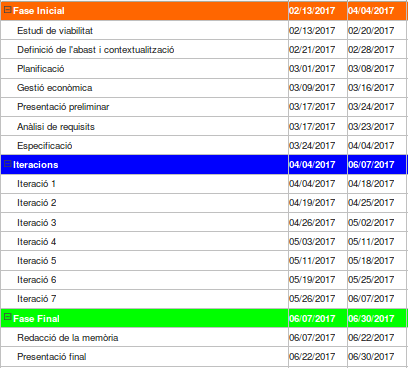
\includegraphics[scale=1]{Figures/ganttFinal.png}
\caption{Taula de planificació final}
\end{figure}

\begin{figure}[!h]
\centering
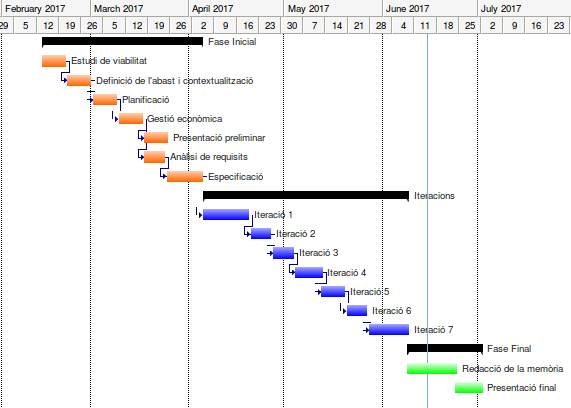
\includegraphics[scale=0.85]{Figures/ganttFinal2.png}
\caption{Diagrama de Gantt final}
\end{figure}

\section{Limitacions i dificultats}
Degut a temes de pressupost, no es pot garantir una quantitat molt gran d'usuaris ja que el servei que s'utilitza per tal d'implementar la base de dades només ofereix una quantitat d'usuaris finita de manera gratuïta. En el cas que es volgués incrementar el nombre d'usuaris s'hauria de comptar amb un pagament mensual al sistema \textit{Firebase}.\\

El mateix passa amb la crida a l'api que retorna la previsió metereològica, aquest servei només permet fer un número finit de crides cada minut. Aquesta limitació però és menys important ja que haurien de registrar-se molts usuaris per tal de sobrecarregar el sistema, i si aquest fos el cas, l'usuari podria tornar a provar d'aconseguir la previsió meterològica uns segons més tard. Cal dir però, que el servei no és molt car i també es podria fer un pagament mensual.\\

A l'inici del projecte es volia oferir l'aplicació a l'usuari en diversos idiomes: català, castellà, anglès i italià. Degut a la limitació temporal del projecte s'ha prioritzat altres tasques i actualment l'aplicació només es pot utilitzar en anglès. També per un tema de prioritats, s'ha posposat el desenvolupament d'una pàgina web informativa sobre l'aplicació mòbil.\\

Els punts que han suposat l'aparició de dificultats han estat, sobretot, la connexió amb els serveis externs que utilitza l'aplicació, ja que no havia treballat mai amb ells; i també la connexió amb la base de dades, que en ser també un servei, aconseguir una connexió que permeti desacoblar al màxim la base de dades ha estat un tema difícil de gestionar. Malgrat aquests obstacles, s'ha pogut tirar el projecte endavant consultant documentació i conversant amb experts en el tema.


\section{Treball futur}

El projecte ha assolit els objectius que es van plantejar a l'inici, tot i així, el sistema pot incorporar més funcionalitats i continuar treballant en diversos aspectes.\\

En primer lloc, com ja s'ha especificat en aquest document l'aplicació està pensada per tal de que sigui molt senzill incorporar noves funcionalitats que donin suport al viatger durant el transcurs del seu viatge. Per aquest motiu, un punt fonamental del treball a fer en un futur és analitzar quines funcionalitats s'utilitzen més i quines es podrien incorporar. Si alguna funcionalitat no s'utilitza s'hauria d'estudiar els motius i actuar. D'atra banda, sempre s'ha d'estar atent a l'aparició de noves tecnologies i sistemes que puguessin millorar el servei.\\

Un altre punt important és crear una versió de l'aplicació per al sistema operatiu \textit{iOS} ja que actualment només està desenvolupat per \textit{Android}. Això permetria que gairebé el 100\% de les persones que utilitzen un \textit{smartphone} poguessin utilitzar l'aplicació.\\

\clearpage

En tercer lloc, degut als meus pocs coneixements en seguretat informàtica seria necessari consultar i valorar quins canvis s'hauria de dur a terme per tal de minimitzar riscs ja que la llei estableix que s'han de protegir les dades. Les mesures de seguretat actuals són molt estàndard.\\


Finalment, es vol treballar en la creació d'una interfície única per la marca WildTraveling, això suposaria contractar especialistes en disseny d'interfícies gràfiques i treballar conjuntament en un disseny nou. Actualment s'utilitzen icones i símbols que, tot i estar lliures de llicència, no són únics del sistema.


